%TDAQ
\clearpage
\section{The Trigger and Data Acquisition}
\label{The_Trigger_and_Data_Acquisition}
The Trigger and Data Acquisition (TDAQ) system of ATLAS decides which events to record and store. As mentioned in Section~\ref{the_lhc}, the 25 ns spacing between proton bunches results in an event rate of 1 GHz, making real-time storage unfeasible.
Since the vast majority of the events aren't interesting for physics analysis here at ATLAS, TDAQ's goal is to reduce the collection rate to 1.5 kHz.
The trigger system is comprised of two triggers: the hardware-based Level 1 Trigger (L1)~\cite{ATLAS:1998ad} and the software-based High Level Trigger (HLT)~\cite{ATLAS:2003aa}.
Figure~\ref{fig:tdaq_layout} illustrates how the system works.

\begin{figure}[ht]
    \centering
    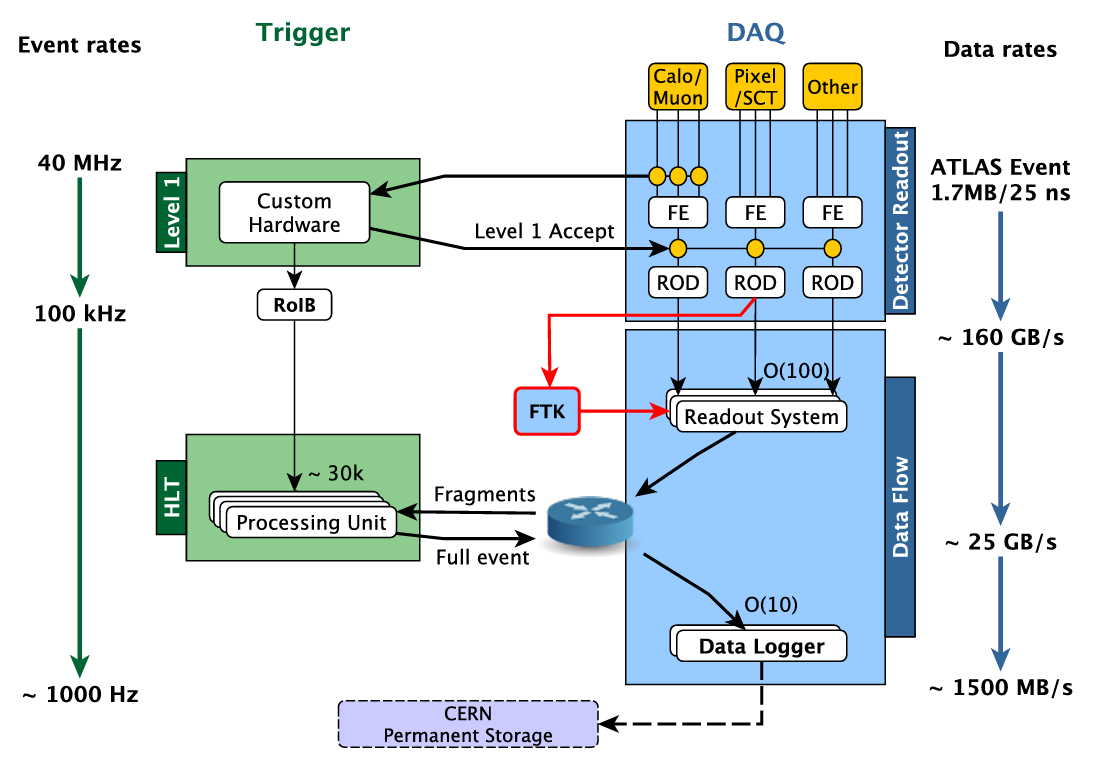
\includegraphics[width=0.85\textwidth]{figures/LHC/tdaq_1.png}
    \caption[]{ATLAS TDAQ Architecture~\cite{Abbott_2016}.}
    \label{fig:tdaq_layout}
\end{figure}

The L1 trigger, directly connected to the muon spectrometer and the calorimeters, identifies physics events with interesting objects such as high-momentum muons, significant missing energy, high-energy electrons/photons, or high-energy hadrons.
The dedicated hardware for the L1 trigger is situated within the same cavern as the ATLAS detector.
Events passing the L1 trigger are transferred from the detectors' Front End (FE) to the Read Out Drivers (ROD) at a reduced the event rate of 100 kHz.

The HLT includes the Level 2 Trigger (L2) and the Event Filter (EF). L1 identifies a region of interest (ROI) of the detector, and the complete event data within this ROI is forwarded to L2. 
``Tracking'' in the ROI is done by L2 to reconstruct the trajectory (or track) of electrically charged particles in the ID.
The tracks and calorimeter information are combined to refine the object selection with higher resolution than what was used in L1, such as tighter requirements on electrons, muons, and missing energy.
Events that pass L2 requirements are sent to the EF, which uses data from the entire detector to decide whether to keep the event.


